\section{Auswertung}
\label{sec:Auswertung}
\subsection{Bestimmung der Fourierkoeffizienten}

\subsection{Untersuchun des Frequenzspektrums}

\subsection{Fourier-Synthese}
Die Oberschwingungen werden nach der Durchführung beschrieben eingestellt.
Die so erhaltenen Bilder sind in Abbildung \ref{fig:eck}, \ref{fig:drei} und \ref{fig:saeg} dargestellt.
\begin{figure}[H]
    \centering
    \caption{Überlagerung der Oberwellen für die Rechteckfunktion.}
    \label{fig:eck}
    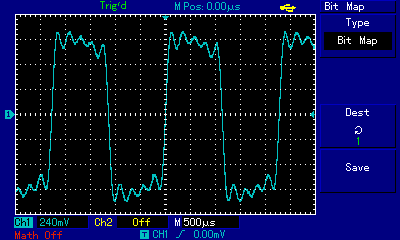
\includegraphics{content/MAP001.png}
\end{figure}
\begin{figure}[H]
    \centering
    \caption{Überlagerung der Oberwellen für die Dreiecksfunktion.}
    \label{fig:drei}
    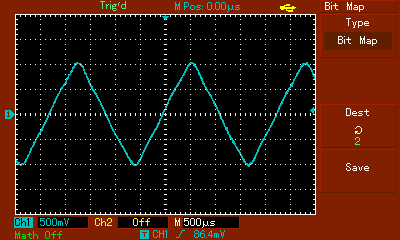
\includegraphics{content/MAP002.png}
\end{figure}
\begin{figure}[H]
    \centering
    \caption{Überlagerung der Oberwellen für die Sägezahnfunktion.}
    \label{fig:saeg}
    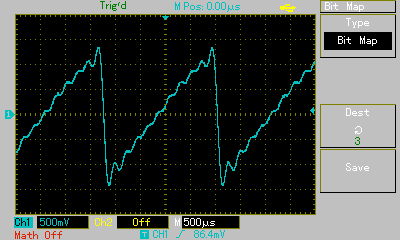
\includegraphics{content/MAP003.png}
\end{figure}
\noindent
Es wurden nur die ersten zehn Oberwellen verwendet um die hier aufgeführten Bilder zu erzeugen.
Die verwendeten Funktion werden durch die Überlagerung der Oberwellen annähernd approximiert.
